%%________________________________________________________________________
%% LEIM | PROJETO
%% 2022 / 2013 / 2012
%% Modelo para relatório
%% v04: alteração ADEETC para DEETC; outros ajustes
%% v03: correção de gralhas
%% v02: inclui anexo sobre utilização sistema controlo de versões
%% v01: original
%% PTS / MAR.2022 / MAI.2013 / 23.MAI.2012 (construído)
%%________________________________________________________________________
\chapter{Tabelas de Requisitos}
\label{ch:tabRequisitos}

\section{Requisitos Funcionais}
Os requisitos estão ordenados de acordo com a sua prioridade.

\begin{table}[h!]
\centering
\begin{tabular}{|l|p{7cm}|l|}
\hline
\textbf{Requisito} & \textbf{Função} & \textbf{Categoria} \\
\hline
R1.1 & Permitir criação de conta - utilizador único & Visível \\
R1.2 & Permitir login & Visível \\
\hline
\end{tabular}
\caption{Requisitos de Autenticação}
\label{tab:requisitosAutenticacao}
\end{table}

\begin{table}[h!]
\centering
\begin{tabular}{|l|p{7cm}|l|}
\hline
\textbf{Requisito} & \textbf{Função} & \textbf{Categoria} \\
\hline
R2.1 & Permitir upload de ficheiros (estritamente do formato .xlsx) & Visível \\
R2.2 & Associar ficheiros carregados a trimestres & Invisível \\
\hline
\end{tabular}
\caption{Requisitos de Gestão de Ficheiros}
\label{tab:requisitosFicheiros}
\end{table}

\begin{table}[h!]
\centering
\begin{tabular}{|l|p{7cm}|l|}
\hline
\textbf{Requisito} & \textbf{Função} & \textbf{Categoria} \\
\hline
R3.1 & Permitir eliminação de ficheiros carregados & Visível \\
R3.2 & Permitir criação de trimestres identificados por 'Quarter N' & Visível \\
R3.3 & Listar todos os trimestres do grupo & Visível \\
\hline
\end{tabular}
\caption{Requisitos de Gestão de Trimestres}
\label{tab:requisitosTrimestres}
\end{table}

\begin{table}[h!]
\centering
\begin{tabular}{|l|p{7cm}|l|}
\hline
\textbf{Requisito} & \textbf{Função} & \textbf{Categoria} \\
\hline
R4.1 & Visualizar gráficos & Visível \\
R4.2 & Aplicar filtros & Visível \\
\hline
\end{tabular}
\caption{Requisitos de Visualização de Dados}
\label{tab:requisitosVisualizacao}
\end{table}

\section{Requisitos Não-Funcionais}
Os requisitos estão ordenados de acordo com a sua prioridade.
\begin{table}[h!]
    \centering
    \begin{tabular}{|l|p{7cm}|l|}
    \hline
    \textbf{Atributo} & \textbf{Detalhe / Restrição - Fronteira} & \textbf{Categoria} \\
    \hline
    Usabilidade & Detalhe - Interface intuitiva & Obrigatório \\
    Usabilidade & Detalhe - Carregamento de gráficos em sem bloquear o utilizador (lazy load) & Obrigatório \\
    Usabilidade & Detalhe - Suporte para múltiplos browsers & Obrigatório \\
    Segurança & Detalhe - Autenticação e Contas & Obrigatório \\
    Segurança & Fronteira - Cada utilizador só pode aceder aos seus dados & Obrigatório \\
    Segurança & Detalhe - Garantir que o sistema só permite ficheiros com formato previsto & Obrigatório \\
    Performance & Detalhe - Suporte para múltiplos utilizadores sem degradação significativa & Desejável \\
    Performance & Detalhe - Resposta rápida às interações do utilizador & Obrigatório \\
    Acessibilidade & Detalhe - Tem de ser navegável por teclado e screen-reader friendly & Obrigatório \\
    Dados & Normalizar os dados que recebe de forma a serem apresentáveis & Obrigatório \\

    \hline
    \end{tabular}
    \caption{Tabela de Requisitos Não Funcionais}
    \label{tab:requisitosNaofuncionais}
    \end{table}
    

\chapter{Casos de Utilização}
\label{ch:casosUtilizacao}

\begin{figure}[h]
\centering
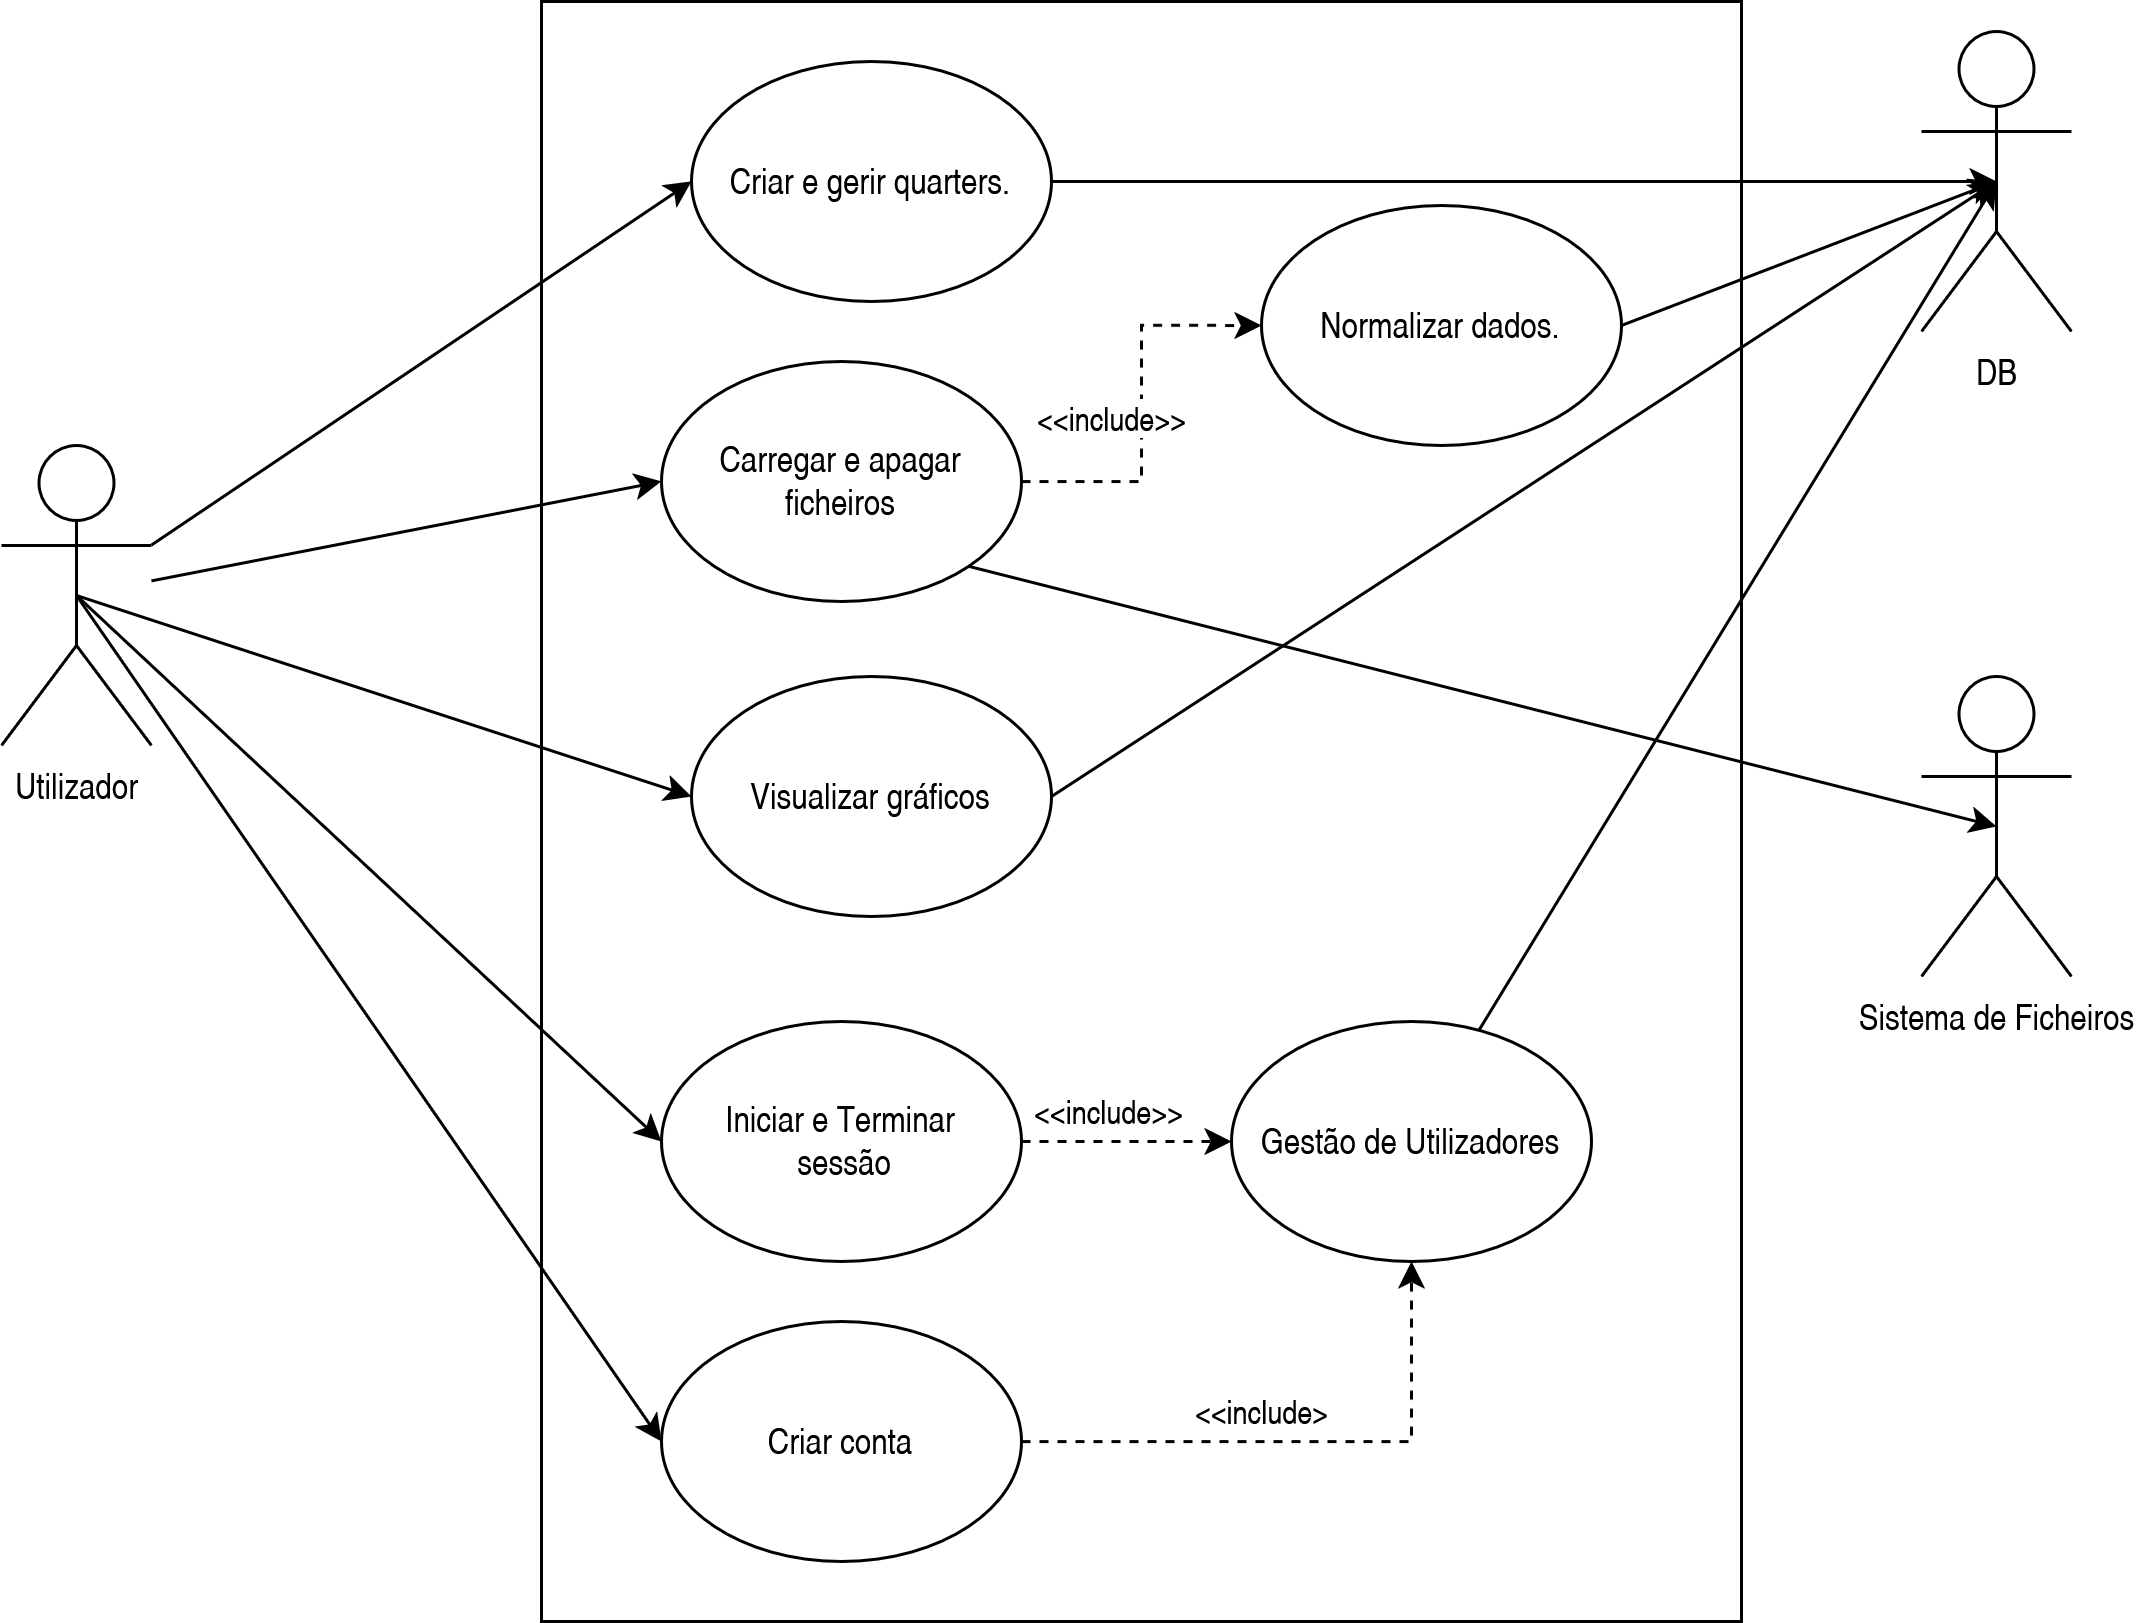
\includegraphics[width=14cm]{./img/usecase_uml}
\caption{\gls{uml} dos Casos de Utilização}
\label{fig:umlCasosUtilizacao}
\end{figure}

\section{Casos de Utilização}

A figura~\ref{fig:umlCasosUtilizacao} apresenta o diagrama UML de casos de utilização da aplicação desenvolvida. Este diagrama ilustra as principais interações entre o utilizador e o sistema, bem como a forma como diferentes componentes externos — nomeadamente a base de dados e o sistema de ficheiros — participam nas operações principais da plataforma.

\begin{figure}[H]
    \centering
    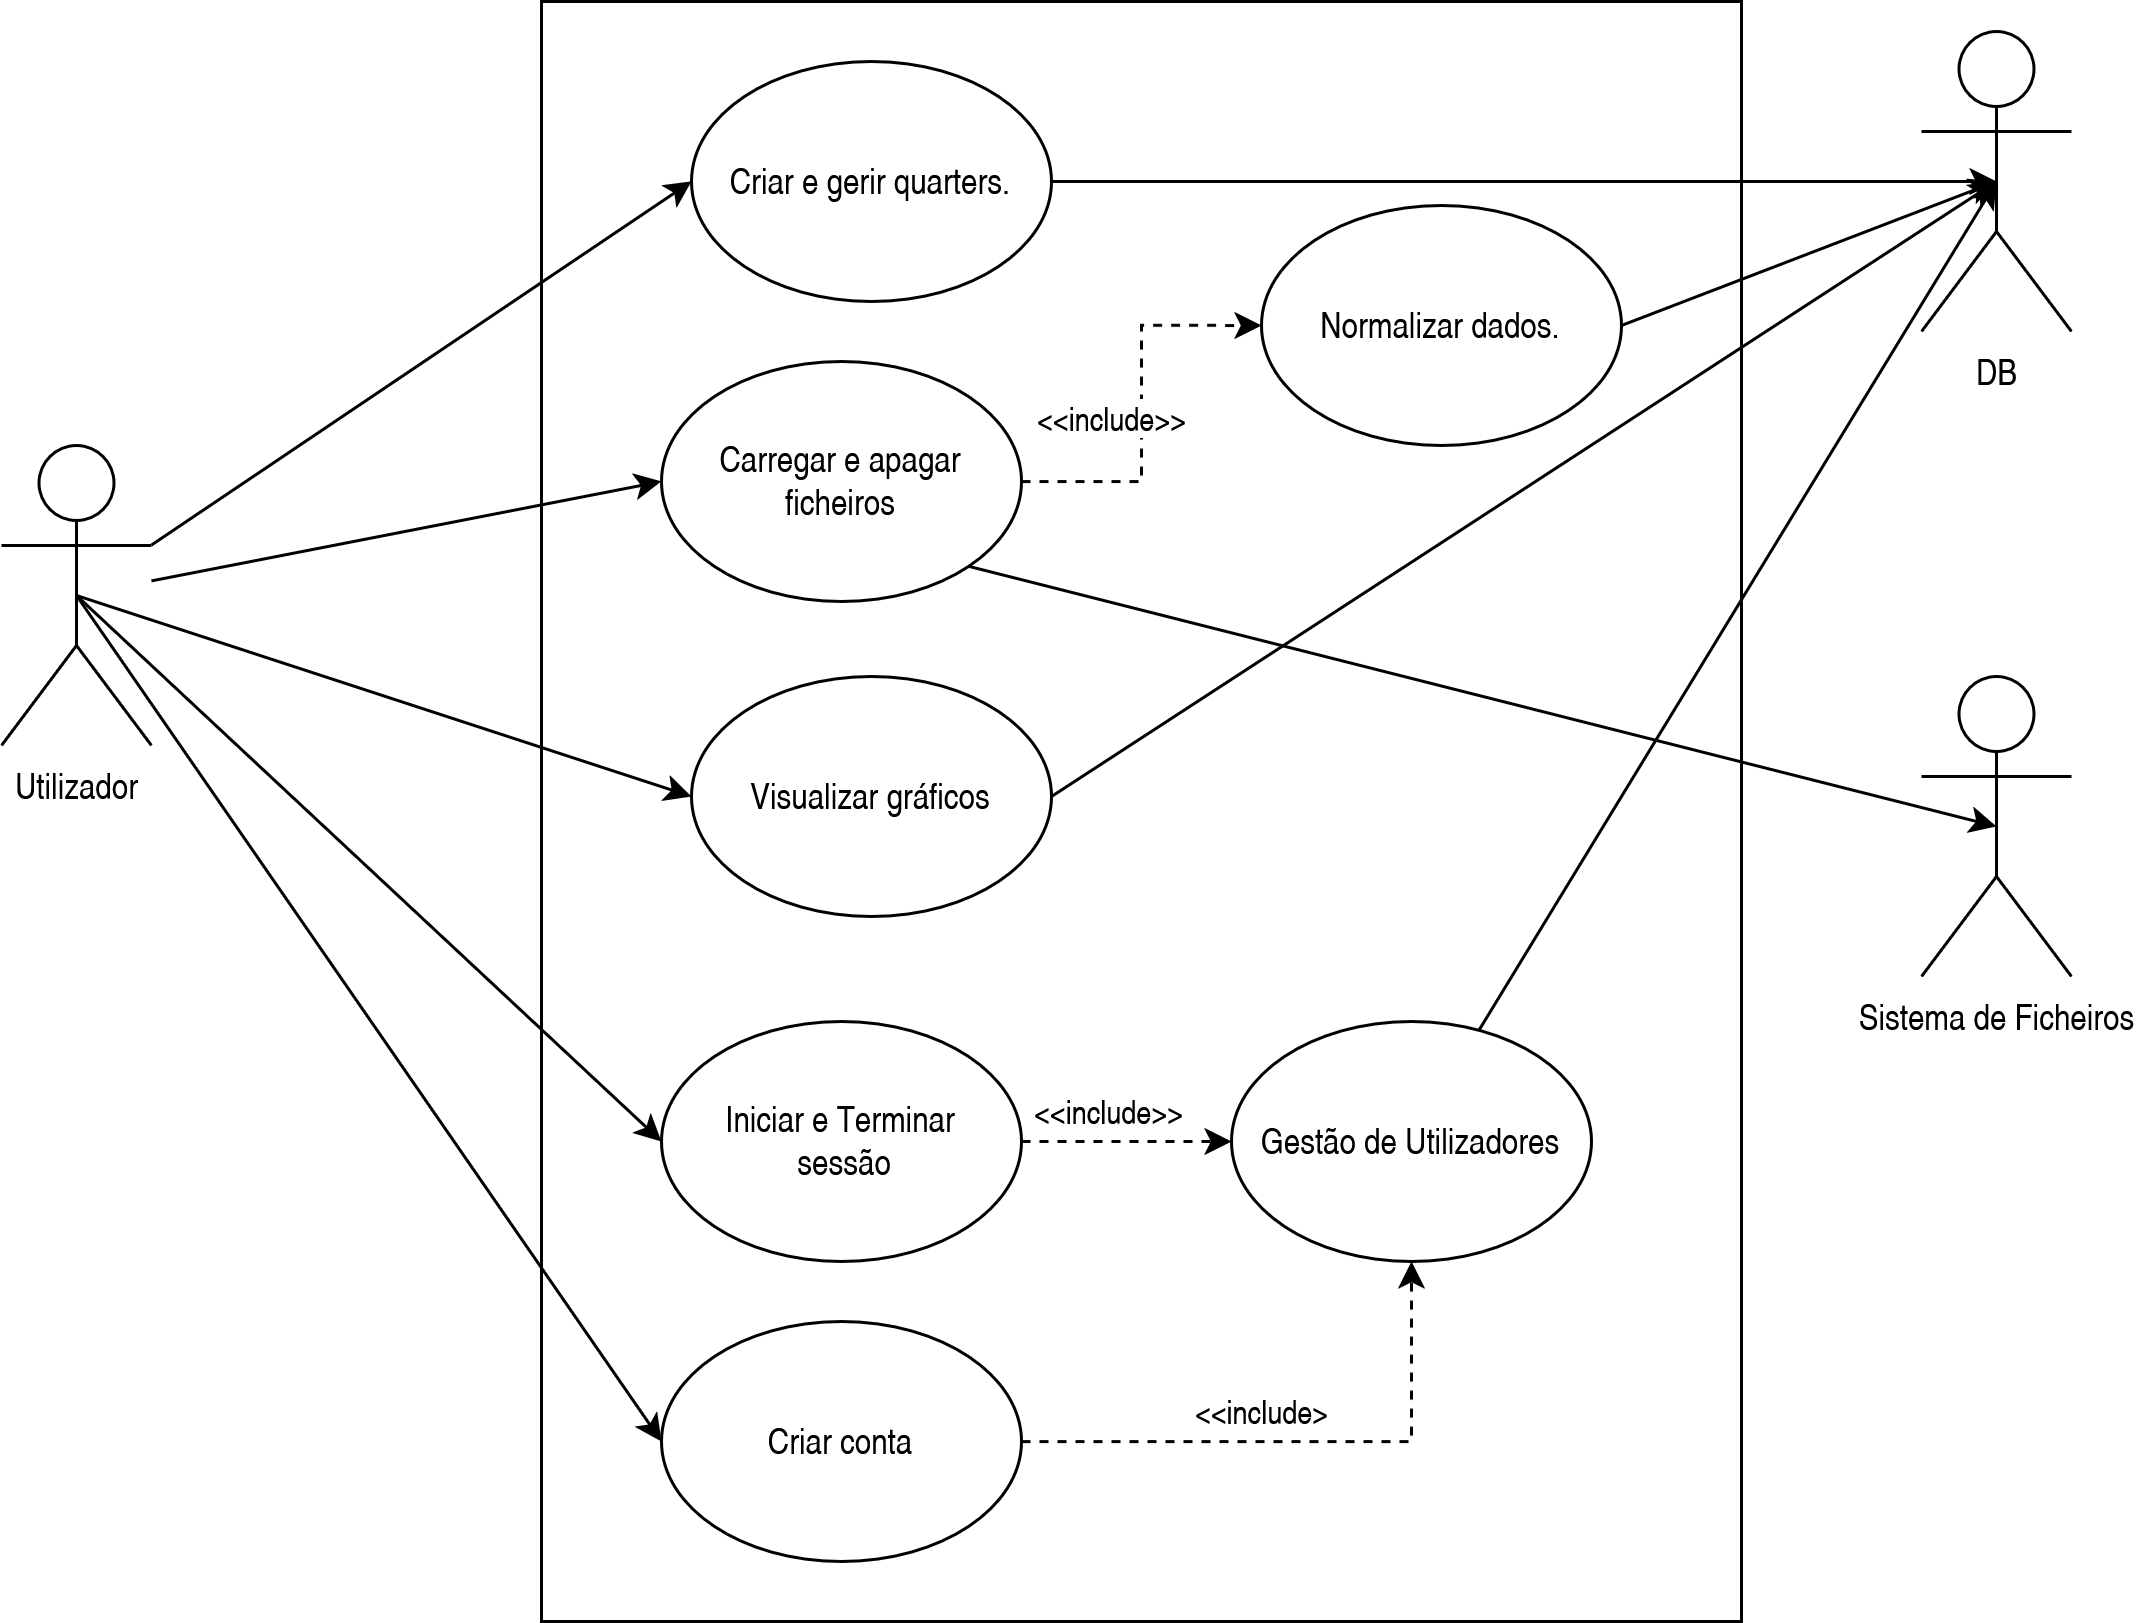
\includegraphics[width=0.9\textwidth]{img/usecase_uml.png}
    \caption{Diagrama de Casos de Utilização do sistema}
    \label{fig:usecase}
\end{figure}

\subsection*{Atores}
\begin{itemize}
    \item \textbf{Utilizador} — É o ator principal, responsável por interagir com o sistema. Pode criar conta, iniciar sessão, carregar ficheiros, visualizar gráficos, entre outras ações.
    \item \textbf{DB (Base de Dados)} — Responsável por armazenar e recuperar dados estruturados, incluindo utilizadores, trimestres, ficheiros processados e metainformação associada.
    \item \textbf{Sistema de Ficheiros} — Componente externo responsável pelo armazenamento físico dos ficheiros carregados e transformados (por exemplo, os CSV resultantes da normalização dos ficheiros Excel).
\end{itemize}

\subsection*{Casos de Utilização}
\begin{itemize}
    \item \textbf{Criar e gerir quarters} — Permite ao utilizador criar unidades lógicas que agrupam os ficheiros por trimestre. Cada quarter é identificado por um UUID e guardado na base de dados.
    \item \textbf{Carregar e apagar ficheiros} — Os utilizadores podem carregar ficheiros XLSX para o sistema, que são automaticamente processados. Também podem remover ficheiros já existentes. Esta operação interage com a base de dados e com o sistema de ficheiros.
    \item \textbf{Normalizar dados} (\textit{include}) — Subprocesso chamado sempre que é feito o carregamento de um ficheiro. Este módulo transforma os dados em formato normalizado (por exemplo, convertendo para CSV, limpando colunas inúteis e ajustando nomes). Comunica diretamente com a base de dados e com o sistema de ficheiros.
    \item \textbf{Visualizar gráficos} — Permite ao utilizador consultar representações gráficas dos dados processados, com suporte a filtros e navegação entre trimestres. Os dados são extraídos dos ficheiros normalizados e da base de dados.
    \item \textbf{Iniciar e terminar sessão} — Processo de autenticação e gestão de sessão do utilizador. Este caso inclui o uso do módulo de \textbf{Gestão de Utilizadores}.
    \item \textbf{Criar conta} — Permite a criação de um novo utilizador no sistema, também incluindo a \textbf{Gestão de Utilizadores}.
    \item \textbf{Gestão de Utilizadores} (\textit{include}) — Caso comum que trata a criação, verificação e autenticação de contas de utilizador. Serve de base a outros casos como iniciar sessão ou registar conta.
\end{itemize}

Este diagrama permite compreender de forma clara as funcionalidades principais da plataforma e a separação de responsabilidades entre os diferentes componentes do sistema.

\chapter{Classificação das folhas \gls{xlsx}}


\chapter{Comparação de gráficos suportados pelo Plotly e Chart.js}
\label{ch:charts}

\begin{table}[H]
\centering
\caption{Comparação de tipos de gráficos suportados por Plotly.js e Chart.js}
\begin{tabular}{|l|c|c|}
\hline
\textbf{Tipo de Gráfico} & \textbf{Plotly.js} & \textbf{Chart.js} \\
\hline
Barras                         & Suportado & Suportado \\
Linhas                         & Suportado & Suportado \\
Dispersão (Scatter)            & Suportado & Suportado \\
Circular (Pie)                 & Suportado & Suportado \\
Área                           & Suportado & Suportado \\
Radar                          & Suportado & Suportado \\
Histograma                     & Suportado & Suportado \\
Box Plot                       & Suportado & Não Suportado \\
Mapa de Calor (Heatmap)        & Suportado & Não Suportado \\
Cascata (Waterfall)            & Suportado & Não Suportado \\
Indicadores (Gauges)           & Suportado & Não Suportado \\
Candlestick (Finanças)         & Suportado & Não Suportado \\
OHLC (Finanças)                & Suportado & Não Suportado \\
Treemap                        & Suportado & Não Suportado \\
Sunburst                       & Suportado & Não Suportado \\
Violin                         & Suportado & Não Suportado \\
Mapa (Geo)                     & Suportado & Não Suportado \\
\hline
\end{tabular}
\label{tab:charts}
\end{table}


\chapter{Cenários Gherkin}
\label{ch:cenariosGherkin}

\begin{verbatim}
Scenario: Creating an account
    Given I access the page 
    And I don't have an account or logged in
    Then I should see the "Create Account" link
    When I click the "Create Account" link
    Then I should be redirected to the "Create Account" form
    And I should see the username field
    And I should see the password filed
    And I should see the confirm password field
    When I fill that form
    And I click "Save"
    Then I should be redirected to the "Login" page
\end{verbatim}



\begin{verbatim}
Background:
	Given that I have an account

Scenario: Login on the app
	When access the website
	And I am not logged in
	Then I should see the Login page
	And I should see the username field
	And I should see the password filed
	When I fill that form with my login details
	And I click "Save"
	Then I should be redirected to the "Home" page
\end{verbatim}
    
\begin{verbatim}
Background:
	Given that I have an account
	And I am logged in on the application

Scenario: Uploading Q1 files
	When I access the "Uploads" page  
	And I click on "Upload files" button 
	Then the upload modal appears 
	When i click on the upload files box
	And I upload all files from Q1 folder
	And I click "Save"
	Then I should see the files that i just uploaded on the page
	When I navigate to the "Home" page
	Then I should see charts. 
	And I should be able to zoom on the chart
	
Scenario: Uploading Q2 files
	When I access the "Uploads" page  
	And I click on "Upload files" button 
	Then the upload modal appears 
	When i click on the upload files box
	And I upload all files from Q2 folder
	And I confirm that the "Quarter Number" has the value of "2".
	And I click "Save"
	Then I should see the files that i just uploaded on the page
	When I navigate to the "Home" page
	Then I should see charts
	And on the "Customer  Needs" chart, i should be able to navigate to Q1.
	And I should be able to zoom on the chart
\end{verbatim}

\begin{verbatim}
    Background:  
	Given that I have an account
	And I am logged in on the application
	And I have uplodaded files to the platform
 
Scenario: Removing a file
	When I navigate to the "Uploads" page  
	Then I should see the files that i already uploaded
	When I click on X button on the file "Customer Needs"
	Then the file is removed from the quarter
	And I should not see charts from that file
	
Scenario: Removing a quarter
	When I navigate to the "Uploads" page  
	Then I should see the files that i already uploaded
	And I should see a "Delete" button.
	When I click on the "Delete" button
	Then I should see all of the files from that section removed 
\end{verbatim}